\chapter{Metodologia}

Um exemplo de utilização de equações matemáticas é apresentado abaixo na Equação~\ref{eq:nome1}:
\begin{equation}
\label{eq:nome1}E=mc^2
\end{equation}

Para um conjunto de equações, como as Equações~\ref{eq:nome2}-\ref{eq:nome3}:
\begin{eqnarray}
\label{eq:nome2} & & \;\;\;\;\; \rho \partial_t v_i
 - \partial_j \tau_{ij} = f_i\\
\label{eq:nome3} & &
\partial_t \tau_{ij}-c_{ijkl}\partial_l v_{k}=-\partial_tg_{ij},
\end{eqnarray}


Um exemplo de utilização de figuras no \LaTeX é apresentado a seguir: na
Figura~\ref{fig:caption1} é mostrado uma figura-exemplo contendo um snapshot
de uma propagação de ondas elásticas em um meio anisotrópico.
\begin{figure}[hbt]
\centering 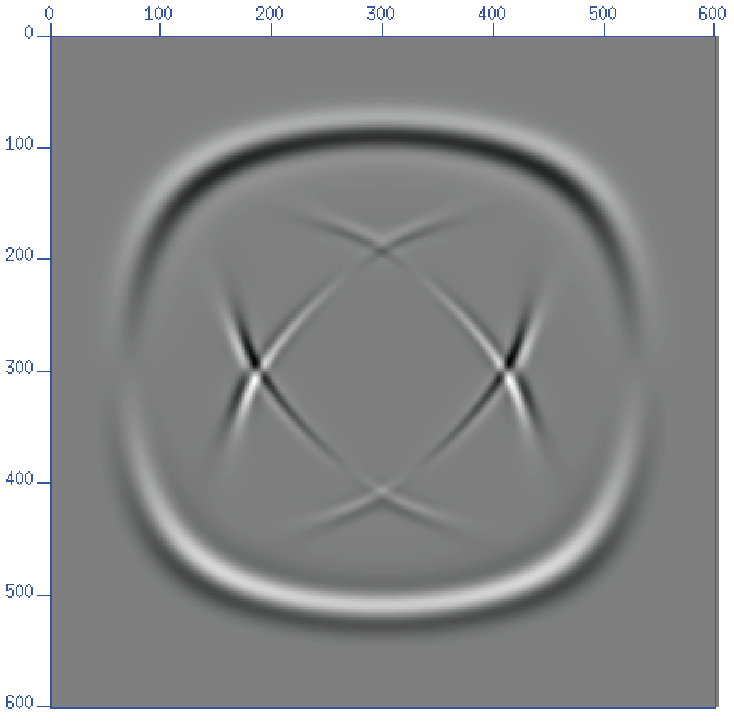
\includegraphics[width=6.5cm,height=6.5cm]{Figs/snap}
\caption[Exemplo de figura simples (texto do índice).]{Exemplo de figura simples:
modelagem elástica de um meio anisotrópico.}
\label{fig:caption1}
\end{figure}

Exemplo de utilização de figuras múltiplas é apresentado na Figura~\ref{fig:cc}
abaixo. Podemos referenciar cada uma das figuras, por exemplo a Figura~\ref{fig:cc_nr} ou
a Figura~\ref{fig:cc_cerjan}.
\begin{figure}[hbt]
\centering \subfigure[Condição de contorno não reflexiva
(CCNR).]{\label{fig:cc_nr}
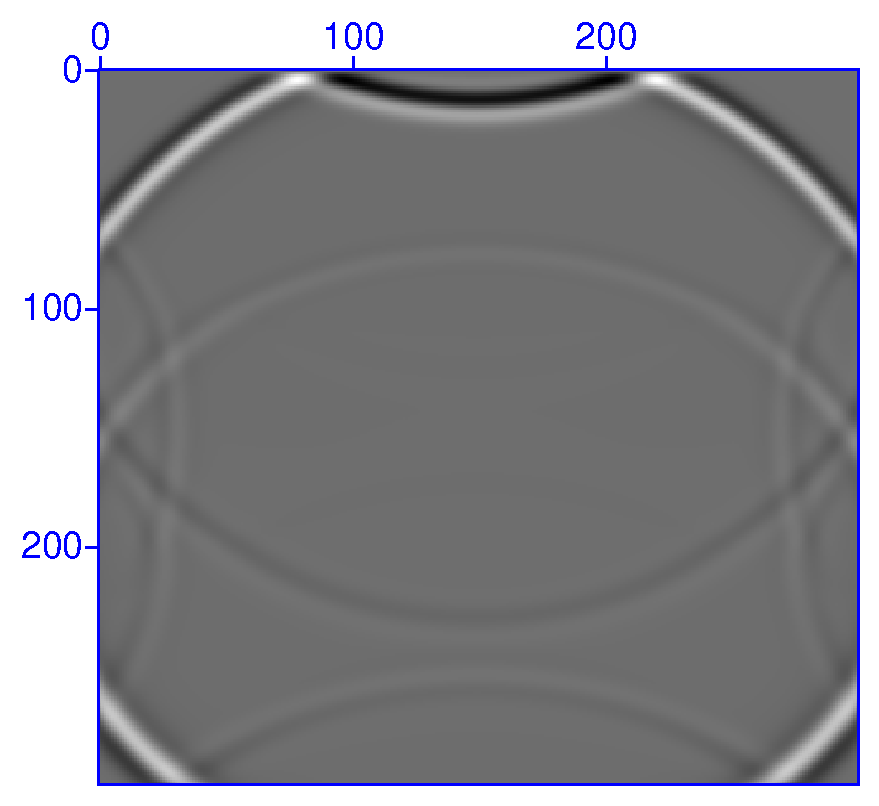
\includegraphics[width=6.5cm,height=6.5cm]
{Figs/cc_nr}} \qquad \subfigure[Camadas de amortecimento +
CCNR.]{\label{fig:cc_cerjan}
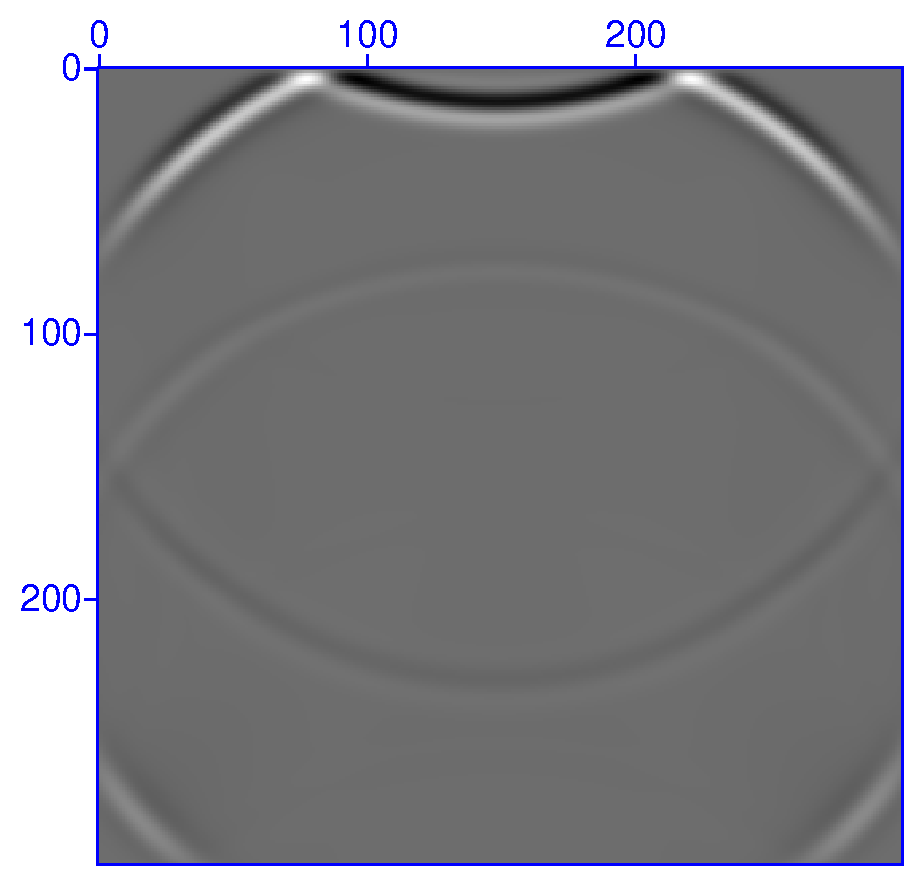
\includegraphics[width=6.5cm,height=6.5cm]{Figs/cerjan}}
\caption[Exemplo de múltiplas figuras (texto do índice).]{Exemplo de múltiplas
figuras: modelagem
acústica mostrando efeito da aplicação da CCNR e camadas de amortecimento
aplicadas nas bordas (menos na superfície). Aplica-se em (a) as CCNR de
Reynolds e em (b) as camadas de amortecimento mais CCNR de Reynolds.}
\label{fig:cc}
\end{figure}

Repare para que o exemplo acima funcione corretamente, é necessário a utilização do pacote``\verb|\usepackage{subfigure}|'', declarado no preambulo do documento principal. Para tal, este pacete deve estar instalado no LaTex utilizado para processar o documento. Indicamos a utilização do MikTex (gratuito) mais atual com editor WinEdt (pago).